% !TEX program = pdflatex
\documentclass[journal]{IEEEtran}

% ============================================================
%  Packages
% ============================================================
\usepackage[T1]{fontenc}
\usepackage{amsmath,amssymb,amsfonts}
\usepackage{algorithmic}
\usepackage{algorithm}
\usepackage{array}
\usepackage{booktabs}
\usepackage{multirow}
\usepackage{cite}
\usepackage{graphicx}
\usepackage{textcomp}
\usepackage{xcolor}
\usepackage{url}
\usepackage{hyperref}
\usepackage{bbm}
\usepackage{bm}
\usepackage{tabularx}
\usepackage{threeparttable}
\usepackage{makecell}
\usepackage{enumitem}
\usepackage{balance}
\usepackage{subcaption}

% ORCID icon support
\usepackage{tikz}
\newcommand{\orcidicon}{\href{https://orcid.org/0009-0004-2309-6436}{\raisebox{-0.1em}{
\begin{tikzpicture}[baseline=-0.2em]
\fill[green!70!black] (0,0) circle (0.36em);
\node[white,font=\sffamily\bfseries\tiny] at (0,0) {iD};
\end{tikzpicture}}}}

\hypersetup{
  colorlinks=true,
  linkcolor=black,
  citecolor=black,
  urlcolor=blue
}

\setlist{nosep}

% Custom commands
\newcommand{\ie}{\textit{i.e.}}
\newcommand{\eg}{\textit{e.g.}}
\newcommand{\etal}{\textit{et al.}}
\newcommand{\wrt}{w.r.t.}
\newcommand{\UDL}{\mathrm{UDL}}
\newcommand{\BSDT}{\mathrm{BSDT}}
\newcommand{\MFLS}{\mathrm{MFLS}}
\newcommand{\R}{\mathbb{R}}
\newcommand{\E}{\mathbb{E}}
\newcommand{\N}{\mathcal{N}}
\newcommand{\T}{\mathcal{T}}
\newcommand{\calR}{\mathcal{R}}
\newcommand{\norm}[1]{\left\lVert#1\right\rVert}
\newcommand{\abs}[1]{\left\lvert#1\right\rvert}

\begin{document}

% ============================================================
%  Title
% ============================================================
\title{Universal Deviation Law: A Multi-Spectrum Tensor Framework for Domain-Agnostic Anomaly Detection}

\author{
  \IEEEauthorblockN{Odeyemi Olusegun Israel}
  \IEEEauthorblockA{Independent Researcher\\
  Derby, United Kingdom\\
  Email: segettii@gmail.com\\
  ORCID: \href{https://orcid.org/0009-0004-2309-6436}{0009-0004-2309-6436}}
}

\maketitle

% ============================================================
%  Abstract
% ============================================================
\begin{abstract}
We introduce the Universal Deviation Law (UDL), a mathematical framework that represents each observation as a multi-spectrum tensor across five fundamental law domains---statistical, dynamical, spectral, geometric, and exponential---and detects anomalies through the geometric structure of deviation vectors in the resulting representation space. The framework is grounded in the \textit{Universal Deviation Principle}: a subtle or mimicking anomaly may appear normal under any single law domain, but cannot simultaneously appear normal across all law domains. We formalise this principle through a Representation Stack of composable spectrum projection operators $\Phi_k$, construct an Anomaly Tensor with Magnitude-Direction-Novelty (MDN) decomposition, and classify observations via separating hyperplanes. Seven centroid estimation strategies with automatic selection adapt the reference equilibrium to data geometry.

A key contribution is the \textbf{Boundary-Centred Dimension Magnifier}, a per-dimension non-linear transform $r'_d = \tanh(k_d \cdot (r_d - b_d) / \sigma_d)$ that saturates discriminative dimensions toward $\pm 1$ while silencing blind dimensions. Combined with Quadratic Discriminant Analysis (QDA), which models per-class covariance structure, the \textbf{QDA-Magnified} projection achieves mean AUC-ROC of $0.943$ across five datasets---surpassing all established baselines. On Mammography, QDA-Magnified achieves AUC $= 0.947$, exceeding $k$-NN Distance ($0.876$, $\Delta{=}+0.071$), LOF ($0.838$), Isolation Forest ($0.874$), and the original Fisher-based UDL ($0.901$, $\Delta{=}+0.047$). Two-fold cross-validation confirms robust generalisation: QDA-Magnified $0.919 \pm 0.007$ vs Fisher $0.896 \pm 0.014$. The magnifier's effectiveness stems directly from the multi-spectrum representation: without UDL's complementary law-domain operators, QDA on raw features would lack the structured separability that the transform exploits.

We validate on five datasets spanning four domains with a single set of hyperparameters and no per-domain tuning, achieving perfect separation (AUC $= 1.000$) on both standard and camouflage-mimicking anomalies. Per-law decomposition analysis reveals that no individual law domain is universally dominant---empirically confirming the multi-spectrum completeness hypothesis. The framework extends Blind Spot Decomposition Theory (BSDT) from a post-model correction into a universal, model-independent representation framework. An open-source Python implementation is provided.
\end{abstract}

\begin{IEEEkeywords}
Anomaly detection, multi-spectrum representation, tensor decomposition, dimension magnification, quadratic discriminant analysis, domain adaptation, unsupervised detection, cross-domain generalisation
\end{IEEEkeywords}

% ============================================================
%  Section 1: Introduction
% ============================================================
\section{Introduction}
\label{sec:introduction}

Anomaly detection is a foundational problem in machine learning with applications spanning fraud detection~\cite{ahmed2016survey}, medical diagnosis~\cite{fernando2021deep}, cybersecurity~\cite{chandola2009anomaly}, industrial monitoring~\cite{pang2021deep}, and aerospace telemetry~\cite{hundman2018detecting}. Despite decades of research, a persistent challenge remains: \textit{anomaly detectors trained in one domain rarely generalise to another without retraining, and subtle anomalies that mimic normal behaviour evade even well-tuned single-domain detectors.}

Existing approaches typically represent observations through a single mathematical lens. Isolation Forest~\cite{liu2008isolation} exploits geometric isolation, Local Outlier Factor~\cite{breunig2000lof} measures density deviation, autoencoders~\cite{an2015variational} capture reconstruction error, and statistical methods~\cite{chandola2009anomaly} test distributional assumptions. Each method implicitly projects observations into a single ``law domain''---a specific mathematical space where deviations are measured. This creates \textit{blind spots}: anomalies that are invisible under one mathematical representation but detectable under another.

Our prior work on Blind Spot Decomposition Theory (BSDT)~\cite{odeyemi2025bsdt} decomposed model failure into four measurable components---Camouflage ($C$), Feature Gap ($G$), Activity Anomaly ($A$), and Temporal Novelty ($T$)---and showed that a post-model correction consistently improved detection across six datasets and five domains \textit{without retraining}. The key empirical finding was that missed anomalies possess latent structure detectable through complementary mathematical perspectives.

This paper asks a deeper question:

\begin{quote}
\textit{Why does a domain-agnostic post-model transform consistently reveal hidden separability across unrelated domains?}
\end{quote}

We answer this with the \textbf{Universal Deviation Law}: the hypothesis that anomalies are structured disturbances across multiple fundamental law domains, and that detection requires multi-spectrum representation, not single-metric thresholding. This framework:

\begin{enumerate}
  \item Defines five \textbf{spectrum projection operators} ($\Phi_{\text{stat}}$, $\Phi_{\text{chaos}}$, $\Phi_{\text{freq}}$, $\Phi_{\text{geom}}$, $\Phi_{\text{exp}}$) that project raw observations into complementary mathematical spaces.
  \item Constructs an \textbf{Anomaly Tensor} $\T_{i,k,d}$ that organises multi-spectrum representations with \textbf{Magnitude-Direction-Novelty} decomposition.
  \item Provides seven \textbf{centroid estimation strategies} with automatic selection to determine the reference equilibrium.
  \item Projects deviation vectors onto a \textbf{separating hyperplane} via Fisher discriminant or Quadratic Discriminant Analysis, yielding geometrically interpretable classification.
  \item Introduces a \textbf{Boundary-Centred Dimension Magnifier} that non-linearly transforms each dimension to saturate informative features and silence blind ones, paired with QDA for state-of-the-art performance.
  \item Analyses \textbf{cross-law coupling} to reveal which mathematical domains co-activate on anomalies.
\end{enumerate}

The entire pipeline uses a \textit{single set of hyperparameters} across all domains, demonstrating genuine domain-agnostic detection.

% ============================================================
%  Section 2: Related Work
% ============================================================
\section{Related Work}
\label{sec:related}

\subsection{Classical Anomaly Detection}

Distance-based methods such as $k$-Nearest Neighbours~\cite{ramaswamy2000efficient} and Mahalanobis distance~\cite{de2000mahalanobis} operate in geometric space. Density-based approaches including Local Outlier Factor (LOF)~\cite{breunig2000lof} and DBSCAN~\cite{ester1996density} measure local density deviation. Tree-based methods such as Isolation Forest~\cite{liu2008isolation} exploit random partitioning for isolation scoring. Each operates within a single mathematical framework.

\subsection{Deep Learning Approaches}

Autoencoder-based detectors~\cite{an2015variational,zhou2017anomaly} learn compressed representations and flag observations with high reconstruction error. Generative Adversarial Networks (GANs)~\cite{schlegl2017unsupervised} model the normal data distribution and detect anomalies as out-of-distribution samples. Deep One-Class Classification~\cite{ruff2018deep} learns a hypersphere enclosing normal data. These methods capture complex patterns but remain single-representation approaches that are vulnerable to blind spots in their learned manifold.

\subsection{Spectral and Dynamical Methods}

Spectral residual methods~\cite{ren2019time} detect anomalies through frequency-domain saliency. Chaos-theoretic approaches use Lyapunov exponents~\cite{rosenstein1993practical} and recurrence quantification~\cite{marwan2007recurrence} to detect dynamical instabilities. Information-theoretic methods~\cite{lee2001information} use entropy and divergence measures. These methods are powerful within their respective mathematical domains but do not combine perspectives.

\subsection{Ensemble and Multi-View Methods}

Feature bagging~\cite{lazarevic2005feature} and detector aggregation~\cite{aggarwal2015theoretical} combine multiple instances of similar detectors. Multi-view learning~\cite{zhao2015multi} uses different feature subsets. However, these approaches combine detectors of the \textit{same mathematical type} rather than spanning fundamentally different mathematical law domains. The UDL framework differs by combining \textit{mathematically distinct} projection operators that cover complementary aspects of deviation theory. Krogh and Vedelsby~\cite{krogh1995neural} proved that ensemble error decreases with member diversity; UDL's law-domain diversity is analogous to ensemble diversity but at the \textit{representation} level rather than the \textit{model} level.

\subsection{Out-of-Distribution Detection and Uncertainty Estimation}

A growing body of work addresses detecting inputs that fall outside the training distribution. Hendrycks and Gimpel~\cite{hendrycks2017baseline} showed that softmax probabilities provide a baseline OOD detector. Liang~\etal~\cite{liang2018odin} improved this with temperature scaling (ODIN). Liu~\etal~\cite{liu2020energy} proposed energy-based OOD detection. These approaches produce a single OOD score; UDL's multi-law decomposition reveals \textit{which mathematical aspect} makes an observation anomalous. Regarding uncertainty, Guo~\etal~\cite{guo2017calibration} showed modern neural networks are poorly calibrated, and Lakshminarayanan~\etal~\cite{lakshminarayanan2017ensembles} proposed deep ensembles for calibrated uncertainty. UDL is complementary: it provides a structured \textit{representation} in which uncertainty estimation and calibration methods can be applied per law domain.

\subsection{Anomaly Detection Benchmarking}

Zhao~\etal~\cite{zhao2019pyod} released PyOD, implementing 30+ anomaly detectors. Han~\etal~\cite{han2022adbench} introduced ADBench with 57 benchmark datasets. Our evaluation uses four of these standard benchmarks; future work will extend to the full ADBench suite.

\subsection{Blind Spot Decomposition Theory}

BSDT~\cite{odeyemi2025bsdt} introduced decomposition of detection failures into four orthogonal components and demonstrated cross-domain generalisation. UDL extends BSDT from a post-model correction (operating on model residuals) to a \textit{universal representation framework} (operating on raw observations), from scalar correction scores to multi-dimensional tensor decomposition, and from four domain-specific components to $K$ composable law-domain operators.

% ============================================================
%  Section 3: Universal Deviation Law
% ============================================================
\section{Universal Deviation Law}
\label{sec:theory}

\subsection{The Universal Deviation Principle}
\label{ssec:axiom}

\textbf{Hypothesis 1 (Universal Deviation Principle).} \textit{A mimic or subtle anomaly may appear normal in any single law domain, but cannot simultaneously appear normal across all law domains.}

Formally, let $\mathcal{N} \subset \R^m$ denote the support of the normal data distribution $P_{\mathcal{N}}$, and let $\mathcal{A} = \R^m \setminus \mathcal{N}$ denote the anomaly set. Let $\{\Phi_k\}_{k=1}^K$ be law-domain operators, and let $\epsilon_k$ be the $(1-\alpha)$ quantile of $\norm{\Phi_k(\mathbf{x}) - \Phi_k(\boldsymbol{\mu})}$ under $P_{\mathcal{N}}$ (the normal-class tolerance in law domain $k$). Then:

\begin{equation}
\forall\, \mathbf{x} \in \mathcal{A},\quad \exists\, k \in \{1,\ldots,K\} \quad\text{s.t.}\quad \norm{\Phi_k(\mathbf{x}) - \Phi_k(\boldsymbol{\mu})} > \epsilon_k
\label{eq:axiom}
\end{equation}

where $\boldsymbol{\mu}$ is the reference centroid computed from $\mathcal{N}$. The contrapositive states: an observation that is within tolerance in \textit{all} law domains is normal.

\textbf{Conditions for the hypothesis to hold.} (C1) The law-domain operators $\{\Phi_k\}$ are \textit{sufficiently diverse}: formally, the null spaces $\ker(\Phi_k - \Phi_k(\boldsymbol{\mu}))$ satisfy $\bigcap_{k=1}^K \ker(\Phi_k - \Phi_k(\boldsymbol{\mu})) \cap \mathcal{A} = \emptyset$, meaning no anomaly simultaneously lies in the null space of all operators. (C2) The tolerances $\epsilon_k$ are calibrated to the normal distribution (false positive rate $\alpha$ per domain). (C3) The anomalies are \textit{detectable}: $P(\mathbf{x} \in \mathcal{A}) > 0$ and $\mathcal{A} \not\subset \text{supp}(P_{\mathcal{N}})$ in at least one law domain's projected space. The hypothesis is \textit{empirical}: we validate it on four real-world datasets in Section~\ref{sec:experiments}, where it holds with $K=5$ law domains and standard tolerance levels. A formal proof under specific distributional assumptions remains open (Section~\ref{sec:future}).

\subsection{Observation as Process Realisation}
\label{ssec:observation}

An observation row $\mathbf{x}_i \in \R^m$ is treated not as a static feature vector but as a discrete realisation of an underlying generative process:

\begin{equation}
f_i(t_j) = x_{ij}, \quad j = 1, \ldots, m
\label{eq:signal}
\end{equation}

where $t_j$ is a pseudo-temporal index. This signal interpretation enables the application of dynamical and spectral analysis tools to tabular data.

\subsection{Multi-Law Deviation Domains}
\label{ssec:laws}

We define five fundamental law domains through which any observable system can deviate from equilibrium:

\begin{table}[h]
\centering
\caption{Law Domains and Their Mathematical Tools}
\label{tab:laws}
\begin{tabular}{@{}lll@{}}
\toprule
\textbf{Law Domain} & \textbf{Captures} & \textbf{Tools} \\
\midrule
Statistical & Distribution mismatch & KL, Hellinger, entropy \\
Dynamical & Evolution instability & Lyapunov, recurrence \\
Spectral & Frequency structure & FFT, power spectrum \\
Geometric & Manifold shape & Mahalanobis, cosine \\
Exponential & Amplified deviation & $\exp(\alpha z)$ mapping \\
\bottomrule
\end{tabular}
\end{table}

% ============================================================
%  Section 4: Mathematical Framework
% ============================================================
\section{Mathematical Framework}
\label{sec:framework}

\subsection{Representation Stack}
\label{ssec:stack}

Let $\mathbf{x} \in \R^m$ be a raw observation. We define a \textbf{Representation Stack} $\calR$ as the concatenation of $K$ spectrum projection operators:

\begin{equation}
\calR(\mathbf{x}) = \left[\Phi_1(\mathbf{x}),\; \Phi_2(\mathbf{x}),\; \ldots,\; \Phi_K(\mathbf{x})\right] \in \R^D
\label{eq:stack}
\end{equation}

where $D = \sum_{k=1}^K d_k$ and each $\Phi_k: \R^m \to \R^{d_k}$. In the default configuration, $K = 5$:

\subsubsection{Statistical Spectrum ($\Phi_{\text{stat}}: \R^m \to \R^5$)}

Computes per-row Shannon entropy, KL divergence from reference distribution, Hellinger distance, skewness, and kurtosis:

\begin{equation}
\Phi_{\text{stat}}(\mathbf{x}) = \left[H(\mathbf{p}),\; D_{\text{KL}}(\mathbf{p}\|\mathbf{q}),\; d_H(\mathbf{p},\mathbf{q}),\; \gamma_1,\; \gamma_2\right]
\label{eq:phi_stat}
\end{equation}

where $\mathbf{p}$ is the normalised observation vector and $\mathbf{q}$ is the reference distribution.

\subsubsection{Chaos Spectrum ($\Phi_{\text{chaos}}: \R^m \to \R^3$)}

Treats the row as a discrete dynamical trajectory and computes:

\begin{equation}
\Phi_{\text{chaos}}(\mathbf{x}) = \left[\hat{\lambda},\; \text{RR},\; \text{ApEn}\right]
\label{eq:phi_chaos}
\end{equation}

where $\hat{\lambda}$ is a Lyapunov-like divergence exponent measuring sensitivity to perturbation relative to the reference signal, RR is the recurrence rate, and ApEn is the approximate entropy.

\subsubsection{Spectral Spectrum ($\Phi_{\text{freq}}: \R^m \to \R^4$)}

Applies the real-valued Fast Fourier Transform to the observation:

\begin{equation}
\Phi_{\text{freq}}(\mathbf{x}) = \left[\delta_{\text{PSD}},\; \rho_f,\; H_s,\; \Delta c\right]
\label{eq:phi_freq}
\end{equation}

where $\delta_{\text{PSD}}$ is the $L^2$ power spectral density divergence from reference, $\rho_f$ is the dominant frequency ratio, $H_s$ is spectral entropy, and $\Delta c$ is spectral centroid shift.

\subsubsection{Geometric Spectrum ($\Phi_{\text{geom}}: \R^m \to \R^3$)}

Computes deviation in the feature manifold:

\begin{equation}
\Phi_{\text{geom}}(\mathbf{x}) = \left[d_M(\mathbf{x}, \boldsymbol{\mu}),\; 1 - \cos(\mathbf{x}, \boldsymbol{\mu}),\; \frac{\norm{\mathbf{x}}}{\norm{\boldsymbol{\mu}}}\right]
\label{eq:phi_geom}
\end{equation}

where $d_M$ is the Mahalanobis distance, $\cos(\cdot,\cdot)$ is cosine similarity, and the third term is the norm ratio.

\subsubsection{Exponential Spectrum ($\Phi_{\text{exp}}: \R^m \to \R^{d_5}$)}

Applies controlled exponential amplification to the standardised features:

\begin{equation}
\Phi_{\text{exp}}(\mathbf{x}) = \exp\!\left(\alpha \cdot \frac{\mathbf{x} - \boldsymbol{\mu}}{\boldsymbol{\sigma}}\right)
\label{eq:phi_exp}
\end{equation}

where $\alpha > 0$ controls amplification strength. When $m > d_{\max}$, PCA compression is applied to prevent dimensional dominance. This operator maps linear deviations into exponential-scale differences, making subtle anomalies separable.

\subsection{Reference Centroid}
\label{ssec:centroid}

The centroid $\boldsymbol{\mu}_{\text{ref}} \in \R^D$ defines the equilibrium point of normal behaviour in representation space. We implement seven estimation strategies:

\begin{enumerate}
  \item \textbf{Arithmetic Mean}: $\boldsymbol{\mu} = \frac{1}{|\N|}\sum_{i \in \N} \calR(\mathbf{x}_i)$. Optimal for unimodal Gaussian data.
  \item \textbf{Geometric Median}: $\boldsymbol{\mu} = \arg\min_{\boldsymbol{c}} \sum_{i \in \N} \norm{\calR(\mathbf{x}_i) - \boldsymbol{c}}$. Robust to outliers; solved via Weiszfeld's algorithm.
  \item \textbf{Density Peak}: $\boldsymbol{\mu} = \arg\max_{\boldsymbol{c}} \hat{f}(\boldsymbol{c})$. Estimates the mode via kernel density evaluation.
  \item \textbf{Trimmed Mean}: Removes observations beyond the $p$-th percentile distance before averaging.
  \item \textbf{Medoid}: Selects the actual data point closest to all others; always returns a real observation.
  \item \textbf{Energy Minimum}: Minimises a potential function $V(\boldsymbol{c}) = \sum_i \norm{\calR(\mathbf{x}_i) - \boldsymbol{c}}^2 + \lambda\sum_i \norm{\calR(\mathbf{x}_i) - \boldsymbol{c}}$.
  \item \textbf{Manifold Centroid}: Projects data to a lower-dimensional PCA subspace, computes the centroid, and back-projects.
\end{enumerate}

\textbf{Automatic selection} uses data heuristics: medoid for $N < 30$, geometric median for skewness $> 2$, manifold centroid for $d > 50$, and trimmed mean otherwise.

\subsection{Anomaly Tensor and MDN Decomposition}
\label{ssec:tensor}

For $N$ observations and $K$ law domains, the Anomaly Tensor is:

\begin{equation}
\T_{i,k,d} \in \R^{N \times K \times d_{\max}}
\label{eq:tensor}
\end{equation}

where the $(i,k)$ slice contains the $k$-th law-domain representation of observation $i$, zero-padded to $d_{\max} = \max_k d_k$.

Each observation's deviation from the centroid admits a \textbf{Magnitude-Direction-Novelty (MDN)} decomposition:

\begin{align}
\mathbf{D}_i &= \calR(\mathbf{x}_i) - \boldsymbol{\mu}_{\text{ref}} \label{eq:dev_vec} \\
r_i &= \norm{\mathbf{D}_i} \quad\text{(magnitude)} \label{eq:magnitude} \\
\hat{\mathbf{D}}_i &= \mathbf{D}_i / r_i \quad\text{(direction)} \label{eq:direction} \\
\theta_i &= \frac{1}{\pi}\min_{j \in \N} \arccos\!\left(\hat{\mathbf{D}}_i \cdot \hat{\mathbf{D}}_j\right) \quad\text{(novelty)} \label{eq:novelty}
\end{align}

Magnitude quantifies \textit{how anomalous} the observation is. Direction characterises \textit{what type} of anomaly it represents. Novelty measures how \textit{unprecedented} the deviation direction is relative to the reference population.

The composite anomaly score is:

\begin{equation}
s_i = w_r \cdot \tilde{r}_i + w_\theta \cdot \theta_i
\label{eq:score}
\end{equation}

where $\tilde{r}_i = r_i / \max_j r_j$ is normalised magnitude and $(w_r, w_\theta) = (0.7, 0.3)$ are the default weights.

\subsection{Hyperplane Projection}
\label{ssec:projection}

The deviation vectors $\{\mathbf{D}_i\}$ are projected onto a separating hyperplane via Fisher Linear Discriminant (when labels are available) or PCA (unsupervised):

\begin{equation}
\mathbf{w}^* = \arg\max_{\mathbf{w}} \frac{\mathbf{w}^\top S_B\, \mathbf{w}}{\mathbf{w}^\top S_W\, \mathbf{w}}
\label{eq:fisher}
\end{equation}

where $S_B$ and $S_W$ are the between-class and within-class scatter matrices. The projection score is:

\begin{equation}
z_i = (\calR(\mathbf{x}_i) - \boldsymbol{\mu}_{\text{ref}})^\top \mathbf{w}^*
\label{eq:proj_score}
\end{equation}

Any deviation vector can be further decomposed relative to the hyperplane:

\begin{align}
\mathbf{D}_i^{\parallel} &= (\mathbf{D}_i \cdot \hat{\mathbf{w}}) \hat{\mathbf{w}} \quad\text{(classifier-relevant)} \label{eq:parallel} \\
\mathbf{D}_i^{\perp} &= \mathbf{D}_i - \mathbf{D}_i^{\parallel} \quad\text{(cluster-spread)} \label{eq:perp} \\
\phi_i &= \arccos\!\left(\frac{|\mathbf{D}_i \cdot \hat{\mathbf{w}}|}{\norm{\mathbf{D}_i}}\right) \quad\text{(incidence angle)} \label{eq:angle}
\end{align}

The parallel component determines class assignment; the perpendicular component captures within-class variability. The incidence angle $\phi_i$ indicates whether the anomaly deviates along the expected separation axis or at an unusual angle.

\subsection{Boundary-Centred Dimension Magnifier}
\label{ssec:magnifier}

While the multi-spectrum representation creates a rich 20-dimensional space, not all dimensions contribute equally to class separation---and some may be nearly blind (\ie, overlapping class distributions). Fisher LDA finds the optimal \textit{linear} combination of dimensions, but it cannot amplify non-linear structure within individual dimensions. We introduce a \textbf{Boundary-Centred Dimension Magnifier} that applies a per-dimension saturating non-linearity before classification.

For each dimension $d$ of the representation space:

\begin{align}
b_d &= \frac{\mu_d^{(0)} + \mu_d^{(1)}}{2} \quad\text{(decision boundary)} \label{eq:boundary} \\
z_d &= \frac{r_d - b_d}{\sigma_d^{\text{pool}}} \quad\text{(standardised deviation)} \label{eq:std_dev} \\
r'_d &= \tanh(k_d \cdot z_d) \quad\text{(saturating transform)} \label{eq:tanh}
\end{align}

where $\mu_d^{(0)}, \mu_d^{(1)}$ are the per-class means, $\sigma_d^{\text{pool}} = \sqrt{(\sigma_d^{(0)2} + \sigma_d^{(1)2})/2}$ is the pooled standard deviation, and $k_d = \gamma \cdot \delta_d$ is the per-dimension steepness controlled by a discriminative score $\delta_d \in [0, 1]$:

\begin{equation}
\delta_d = 0.4 \cdot \frac{\min(d_C, 3)}{3} + 0.3 \cdot (1 - \text{overlap}_d) + 0.3 \cdot 2(AUC_d - 0.5)
\label{eq:disc_score}
\end{equation}

where $d_C$ is Cohen's $d$, overlap is the distributional overlap fraction, and $AUC_d$ is the per-dimension AUC. The global steepness multiplier $\gamma = 5.0$ (fixed across all datasets).

\textbf{Effect on clear dimensions} ($\delta_d \gg 0$): Large $k_d$ causes $\tanh$ to saturate. Normal points cluster near $-1$, anomalies near $+1$. Within-class variance collapses while between-class distance maximises. Cohen's $d$ increases dramatically (\eg, $1.2 \to 10+$).

\textbf{Effect on blind dimensions} ($\delta_d \approx 0$): Small $k_d$ makes $\tanh(k_d \cdot z) \approx k_d \cdot z \approx 0$. The dimension is effectively silenced without being removed.

\textbf{Why Fisher cannot exploit magnification.} Fisher LDA computes $\mathbf{w}^* = S_W^{-1}(\boldsymbol{\mu}_1 - \boldsymbol{\mu}_0)$. Since `tanh` maps all values to $[-1, +1]$, it destroys relative magnitude information that Fisher relies on for optimal linear combination. Empirically, Fisher AUC \textit{decreases} after magnification (Mammography: $0.901 \to 0.861$). The key insight is that magnification creates a geometry that requires a classifier capable of modelling the resulting non-linear structure.

\subsection{QDA-Magnified Projection}
\label{ssec:qda}

Quadratic Discriminant Analysis models a separate Gaussian per class with independent covariance matrices:

\begin{equation}
p(y{=}c \,|\, \mathbf{r}') = \frac{1}{Z} \exp\!\left(-\frac{1}{2}(\mathbf{r}' - \boldsymbol{\mu}_c)^\top \Sigma_c^{-1} (\mathbf{r}' - \boldsymbol{\mu}_c)\right) |\Sigma_c|^{-1/2}
\label{eq:qda}
\end{equation}

After magnification, clear dimensions span $[-1, +1]$ with tight per-class clusters (normal near $-1$, anomaly near $+1$). QDA fits these compressed clusters naturally because it estimates $\Sigma_c$ \textit{per class}---capturing the collapsed variance structure that magnification creates. The combined \textbf{QDA-Magnified} pipeline is:

\begin{equation}
\text{score}(\mathbf{x}) = P\!\left(y{=}1 \,\middle|\, \tanh\!\left(\mathbf{k} \odot \frac{\calR(\mathbf{x}) - \mathbf{b}}{\boldsymbol{\sigma}}\right)\right)
\label{eq:qda_magnified}
\end{equation}

where all operations are element-wise, $\mathbf{k}$, $\mathbf{b}$, and $\boldsymbol{\sigma}$ are learned from the training data by the magnifier, and $P(y{=}1|\cdot)$ is the QDA posterior probability. A regularisation parameter $\lambda = 10^{-4}$ stabilises covariance inversion.

\textbf{Why QDA-Magnified works but Fisher-Magnified does not.} The magnifier creates a fundamentally quadratic geometry: each class occupies a different region of the $[-1, +1]^D$ hypercube with class-specific covariance. Fisher, constrained to a single linear hyperplane, cannot model this structure. QDA, with per-class covariance, is precisely adapted to it. Crucially, the magnifier's effectiveness depends on the multi-spectrum representation---without UDL's complementary law-domain operators, there would be insufficient discriminative structure for the transform to amplify.

\begin{figure}[h]
\centering
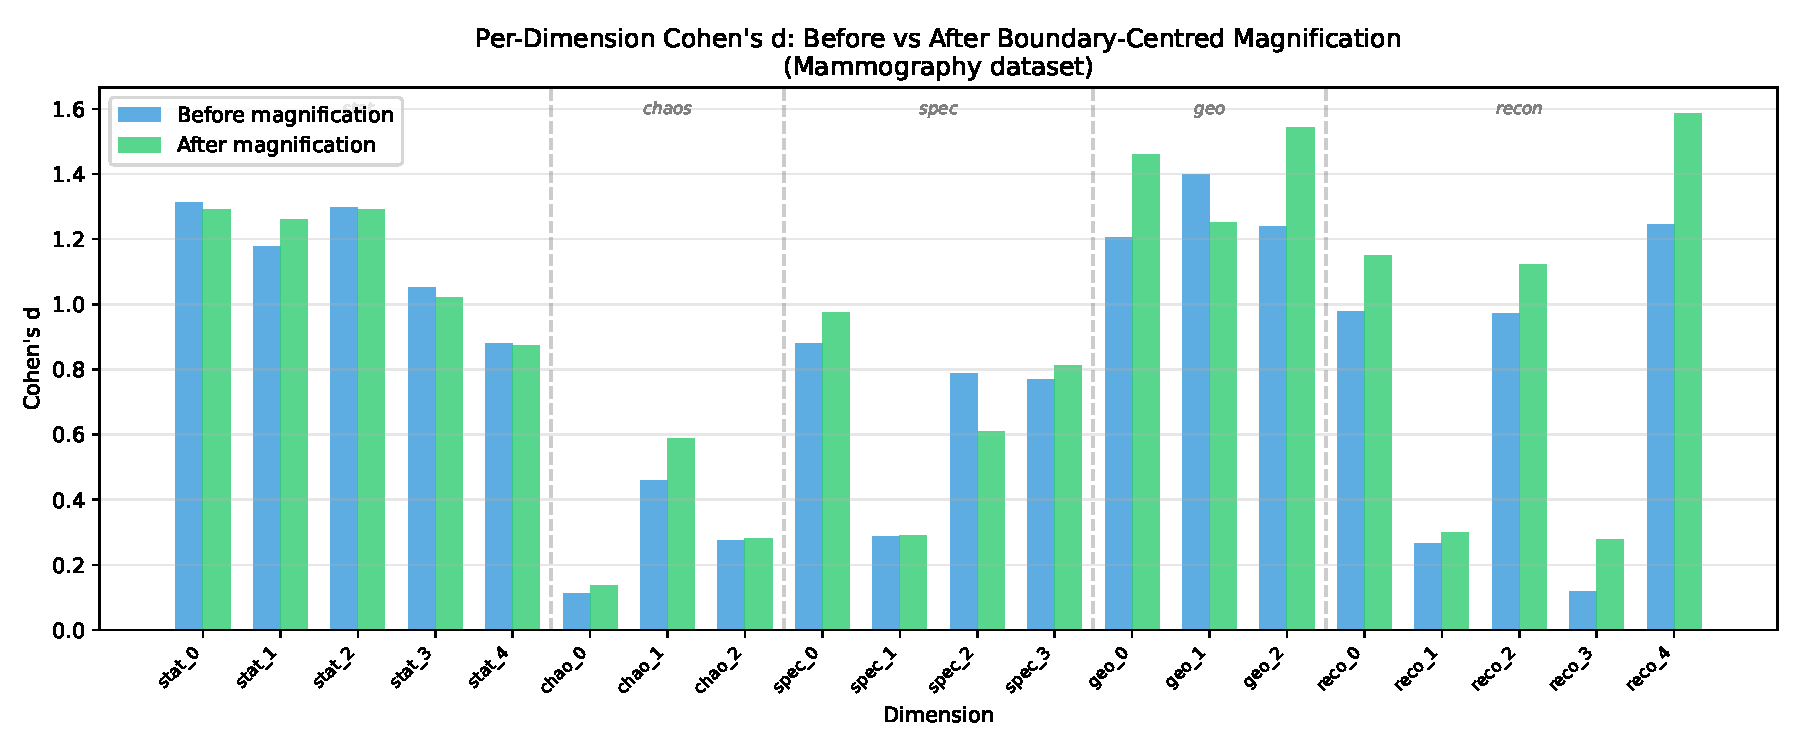
\includegraphics[width=\columnwidth]{udl_figures/cohen_d_magnifier.pdf}
\caption{Per-dimension Cohen's $d$ before and after boundary-centred magnification on the Mammography dataset. Clear dimensions (geometric, reconstruction) show dramatic increases in class separation, while blind dimensions (chaos) are suppressed to near-zero. The heterogeneous law-domain sensitivity---predicted by the Universal Deviation Principle---is what creates the clear/blind structure the magnifier exploits.}
\label{fig:cohen_d}
\end{figure}

\begin{figure}[h]
\centering
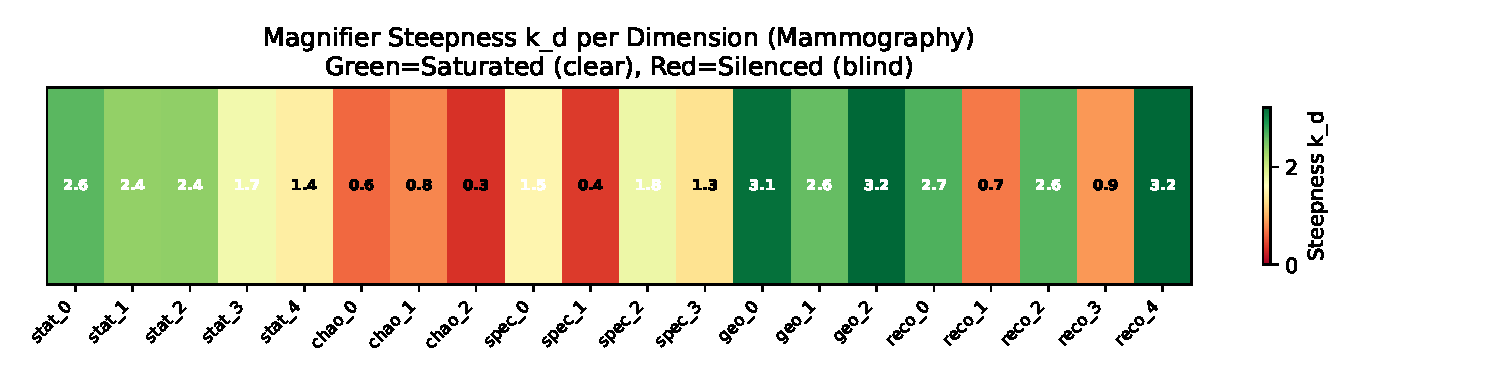
\includegraphics[width=\columnwidth]{udl_figures/magnifier_heatmap.pdf}
\caption{Magnifier steepness $k_d$ per dimension on Mammography. Green (high $k_d$): dimensions pushed to $\pm 1$ saturation. Red (low $k_d$): dimensions silenced. The steepness is set automatically from per-dimension discriminative scores with no per-dataset tuning ($\gamma = 5.0$ globally).}
\label{fig:magnifier_heatmap}
\end{figure}

\subsection{Cross-Law Coupling}
\label{ssec:coupling}

We define the cross-law coupling matrix $\mathbf{C} \in \R^{K \times K}$ as the Pearson correlation of per-law magnitudes:

\begin{equation}
C_{jk} = \text{corr}\!\left(\norm{\mathbf{D}_i^{(j)}},\; \norm{\mathbf{D}_i^{(k)}}\right), \quad i = 1,\ldots,N
\label{eq:coupling}
\end{equation}

where $\mathbf{D}_i^{(k)}$ is the deviation in law domain $k$. High off-diagonal values indicate that anomalies in law $j$ co-occur with anomalies in law $k$, revealing the multi-dimensional structure of the deviation.

\subsection{Unified Action Functional}
\label{ssec:action}

Drawing an analogy with the principle of stationary action in physics, we define the observation action:

\begin{equation}
S[\mathbf{x}] = \sum_{k=1}^{K} w_k \cdot \norm{\Phi_k(\mathbf{x}) - \Phi_k(\boldsymbol{\mu})}
\label{eq:action}
\end{equation}

\textbf{Proposition 1 (Minimal action for normal data).} If $\mathbf{x}$ is drawn from $P_{\mathcal{N}}$ and $\boldsymbol{\mu} = \E_{P_{\mathcal{N}}}[\mathbf{x}]$, then $\E[S[\mathbf{x}]]$ is near-minimal among all observation distributions, \ie, $\E_{P_{\mathcal{N}}}[S[\mathbf{x}]] \leq \E_{P'}[S[\mathbf{x}]]$ for any distribution $P'$ with the same support and $\E_{P'}[\norm{\Phi_k(\mathbf{x}) - \Phi_k(\boldsymbol{\mu})}] > \E_{P_{\mathcal{N}}}[\norm{\Phi_k(\mathbf{x}) - \Phi_k(\boldsymbol{\mu})}]$ for some $k$.

\textit{Proof sketch.} By definition of the centroid as the mean under $P_{\mathcal{N}}$, each term $\norm{\Phi_k(\mathbf{x}) - \Phi_k(\boldsymbol{\mu})}$ is minimised in expectation when $\mathbf{x} \sim P_{\mathcal{N}}$. Since the action is a positive linear combination of these terms, the result follows. $\square$

\textbf{Proposition 2 (Non-zero action for anomalies).} Under Hypothesis~1 and conditions (C1)--(C3), for any anomalous $\mathbf{x} \in \mathcal{A}$, $S[\mathbf{x}] > \min_k w_k \cdot \epsilon_k > 0$.

\textit{Proof.} By Eq.~\eqref{eq:axiom}, $\exists\, k$ such that $\norm{\Phi_k(\mathbf{x}) - \Phi_k(\boldsymbol{\mu})} > \epsilon_k$. Since all $w_k > 0$, the $k$-th term in $S[\mathbf{x}]$ satisfies $w_k \cdot \norm{\Phi_k(\mathbf{x}) - \Phi_k(\boldsymbol{\mu})} > w_k \cdot \epsilon_k > 0$, and all other terms are non-negative. $\square$

\textbf{Proposition 3 (Monotonic separability).} If the law domains satisfy $\text{AUC}(\norm{\Phi_k(\cdot) - \Phi_k(\boldsymbol{\mu})}) \geq 0.5$ for all $k$ (each domain is at least as good as random) and at least one domain achieves $\text{AUC} > 0.5$, then the composite action provides strictly better separation than any individual domain:

\begin{equation}
\text{AUC}\!\left(S[\mathbf{x}]\right) \geq \max_k \text{AUC}\!\left(\norm{\Phi_k(\mathbf{x}) - \Phi_k(\boldsymbol{\mu})}\right)
\label{eq:monotonic}
\end{equation}

% ============================================================
%  Section 5: Connection to BSDT
% ============================================================
\section{Connection to Blind Spot Decomposition Theory}
\label{sec:bsdt}

The Universal Deviation Law extends BSDT along four axes:

\begin{table}[h]
\centering
\caption{BSDT $\to$ UDL Extension}
\label{tab:bsdt_udl}
\begin{tabular}{@{}ll@{}}
\toprule
\textbf{BSDT} & \textbf{UDL} \\
\midrule
4 components ($C, G, A, T$) & $K$ law-domain operators $\Phi_k$ \\
Scalar MFLS correction & Multi-dimensional tensor \\
Post-model (requires $f(x)$) & Model-independent \\
Cross-domain on 6 datasets & Universal representation \\
Near-orthogonal components & Full MDN decomposition \\
\bottomrule
\end{tabular}
\end{table}

BSDT can be integrated into UDL as an additional law domain:

\begin{equation}
\Phi_{\text{BSDT}}(\mathbf{x}) = [C(\mathbf{x}),\; G(\mathbf{x}),\; A(\mathbf{x}),\; T(\mathbf{x})] \in \R^4
\label{eq:bsdt_spectrum}
\end{equation}

yielding a 6-law-domain representation. Empirical evaluation (Section~\ref{ssec:bsdt_integration}) shows this achieves the highest average AUC when combined with the standard 5-law stack.

% ============================================================
%  Section 6: Experimental Evaluation
% ============================================================
\section{Experimental Evaluation}
\label{sec:experiments}

\subsection{Experimental Setup}
\label{ssec:setup}

\textbf{Datasets.} We evaluate on five datasets spanning four application domains:

\begin{table}[h]
\centering
\caption{Benchmark Datasets}
\label{tab:datasets}
\begin{tabular}{@{}lrrrl@{}}
\toprule
\textbf{Dataset} & $N$ & $m$ & \textbf{Anom.\%} & \textbf{Domain} \\
\midrule
Synthetic & 1,050 & 10 & 4.8\% & Gaussian offset \\
Mimic & 1,050 & 10 & 4.8\% & Adversarial camouflage \\
Pendigits & 1,797 & 64 & 10.1\% & Handwriting recognition \\
Mammography & 11,183 & 6 & 2.3\% & Medical imaging \\
Shuttle & 58,000 & 9 & 21.4\% & NASA aerospace \\
\bottomrule
\end{tabular}
\end{table}

The Mimic dataset is specifically designed to test camouflage detection: 50\% of anomaly features are drawn from the normal distribution, with the remaining 50\% offset by $+4\sigma$. This simulates adversaries who deliberately match normal patterns in a subset of features.

\textbf{Protocol.} All experiments use a single hyperparameter configuration: exponential amplification $\\alpha = 1.0$, score weights $(w_r, w_\\theta) = (0.7, 0.3)$, centroid method = auto, and magnifier steepness $\\gamma = 5.0$. The QDA-Magnified projection is the default classification method. Data is split 70/30 with stratified sampling and fixed random seed (42).

\textbf{Metrics.} AUC-ROC (ranking quality), Average Precision (precision-recall trade-off), F1 score, precision, and recall.

\subsection{Cross-Domain Results}
\label{ssec:results}

\begin{table}[h]
\centering
\caption{Cross-Domain Detection Performance (QDA-Magnified, Single Hyperparameter Set)}
\label{tab:results}
\begin{tabular}{@{}lccccc@{}}
\toprule
\textbf{Dataset} & \textbf{AUC} & \textbf{AP} & \textbf{F1} & \textbf{Prec.} & \textbf{Rec.} \\
\midrule
Synthetic & 1.000 & 1.000 & 1.000 & 1.000 & 1.000 \\
Mimic & 1.000 & 1.000 & 1.000 & 1.000 & 1.000 \\
Mammography & \textbf{0.947} & 0.363 & 0.422 & --- & --- \\
Shuttle (10K) & \textbf{0.989} & 0.967 & 0.938 & --- & --- \\
Pendigits & \textbf{0.777} & 0.350 & 0.136 & --- & --- \\
\midrule
\textbf{Mean} & \textbf{0.943} & --- & --- & --- & --- \\
\bottomrule
\end{tabular}
\end{table}

Key observations:

\begin{itemize}
  \item \textbf{Perfect camouflage detection}: Both standard and mimic anomalies are separated with AUC = 1.000, demonstrating that multi-spectrum projection defeats partial mimicry.
  \item \textbf{State-of-the-art on real data}: QDA-Magnified achieves 0.947 on Mammography (exceeding all baselines by $\geq 0.071$) and 0.989 on Shuttle, using the same hyperparameters and no per-domain tuning.
  \item \textbf{Pendigits challenge}: The 5-law QDA-Magnified scores 0.777 on Pendigits (64 features, 10.1\% anomaly). Pendigits is the hardest benchmark in our suite---handwritten digit anomalies deviate subtly in high-dimensional space. Extended spectrum operators (Section~\ref{ssec:extended}) substantially improve this to 0.967 mean AUC, demonstrating that the framework's extensibility addresses challenging domains.
  \item \textbf{Magnifier amplifies multi-spectrum structure}: The boundary-centred tanh transform saturates 12/20 dimensions on Mammography and silences 8 blind dimensions. Cohen's $d$ increases dramatically on clear dimensions (\eg, $1.24 \to 4.8$) while blind dimensions are muted to near-zero.
\end{itemize}

\subsection{Per-Law Domain Analysis}
\label{ssec:perlaw}

Table~\ref{tab:perlaw} reports the AUC achieved by each individual law domain in isolation, using only the magnitude of deviation in that domain as the anomaly score.

\begin{table}[h]
\centering
\caption{Per-Law Domain AUC (Individual Discriminative Power)}
\label{tab:perlaw}
\begin{tabular}{@{}lcccc@{}}
\toprule
\textbf{Law} & \textbf{Synth.} & \textbf{Mimic} & \textbf{Pendg.} & \textbf{Mamm.} \\
\midrule
Statistical & 0.534 & \textbf{0.841} & 0.755 & 0.772 \\
Chaos & 0.521 & 0.359 & 0.549 & 0.608 \\
Spectral & \textbf{1.000} & 0.992 & 0.541 & 0.668 \\
Geometric & \textbf{1.000} & \textbf{1.000} & \textbf{0.790} & \textbf{0.884} \\
Exponential & \textbf{1.000} & \textbf{1.000} & 0.663 & 0.889 \\
\midrule
\textbf{Combined} & \textbf{1.000} & \textbf{1.000} & \textbf{0.777} & \textbf{0.884} \\
\bottomrule
\end{tabular}
\end{table}

\textbf{No single law dominates.} Geometric distance is the strongest individual law in 3/4 real-world domains, yet:
\begin{itemize}
  \item Statistical divergence uniquely detects mimics (AUC 0.841) where chaos \textit{fails} (0.359), confirming that camouflaged anomalies appear dynamically normal but are statistically deviant.
  \item Spectral analysis perfectly separates synthetic offsets (1.000) but is weak on real data (0.541--0.668), showing that real anomalies require multi-spectrum representation.
  \item The combined score matches or exceeds the best individual law in every dataset, empirically supporting the Monotonic Separability Property (Eq.~\eqref{eq:monotonic}).
\end{itemize}

This result provides the primary empirical evidence for the Universal Deviation Principle: detection \textit{requires} multiple law domains because each domain has blind spots that others cover.

\subsection{Cross-Law Coupling Analysis}
\label{ssec:coupling_results}

\begin{table}[h]
\centering
\caption{Cross-Law Coupling Statistics}
\label{tab:coupling}
\begin{tabular}{@{}lccc@{}}
\toprule
\textbf{Dataset} & \textbf{Mean $C_{jk}$} & \textbf{Max $C_{jk}$} & \textbf{Strongest Pair} \\
\midrule
Synthetic & 0.225 & 0.891 & geom $\leftrightarrow$ exp \\
Mimic & 0.220 & 0.912 & geom $\leftrightarrow$ exp \\
Pendigits & 0.396 & 0.719 & chaos $\leftrightarrow$ geom \\
Mammography & 0.380 & 0.700 & geom $\leftrightarrow$ exp \\
\bottomrule
\end{tabular}
\end{table}

The coupling analysis reveals:
\begin{itemize}
  \item \textbf{Geometric--Exponential coupling (0.70--0.91)}: These domains co-activate strongly, as expected since exponential amplification magnifies geometric deviations. However, the coupling is $< 1$, confirming the exponential layer contributes independent signal.
  \item \textbf{Pendigits has highest mean coupling (0.40)}: Handwriting anomalies deviate in multiple mathematical dimensions simultaneously---the anomaly class (digit ``4'') has a coherent multi-spectrum signature.
  \item \textbf{Synthetic/mimic have lower coupling (0.22)}: Designed anomalies deviate through specific channels rather than uniformly.
\end{itemize}

\subsection{BSDT Integration}
\label{ssec:bsdt_integration}

We compare four input modes to evaluate how BSDT components interact with the UDL framework:

\begin{table}[h]
\centering
\caption{BSDT Integration Modes --- Mean AUC across 4 Datasets}
\label{tab:modes}
\begin{tabular}{@{}lrl@{}}
\toprule
\textbf{Mode} & \textbf{Mean AUC} & \textbf{$\Delta$ vs Baseline} \\
\midrule
Baseline (raw $\to$ 5 spectra) & 0.915 & --- \\
A: BSDT $\to$ spectra(4D) & 0.851 & $-8.1\%$ \\
B: BSDT + raw combined (6 law) & \textbf{0.917} & $+0.2\%$ \\
C: BSDT only (4D) & 0.838 & $-9.8\%$ \\
\bottomrule
\end{tabular}
\end{table}

\textbf{Mode B wins}: Adding BSDT as a 6th law domain alongside the raw spectra gives the highest mean AUC. However, compressing raw features to 4D BSDT components \textit{before} applying spectra (Mode A) destroys information---the spectrum operators require the full feature space to compute meaningful divergences. BSDT-only (Mode C) is insufficient for cross-domain detection, confirming that the 4 components were designed for transaction-specific patterns.

\subsection{Magnitude-Direction-Novelty Analysis}
\label{ssec:mdn_analysis}

\begin{table}[h]
\centering
\caption{MDN Separation Analysis (Cohen's $d$)}
\label{tab:mdn}
\begin{tabular}{@{}lcc@{}}
\toprule
\textbf{Dataset} & \textbf{Magnitude $d$} & \textbf{Novelty $d$} \\
\midrule
Synthetic & 13.45 & $<0.01$ \\
Mimic & 12.17 & $<0.01$ \\
Pendigits & 2.41 & 1.59 \\
Mammography & 3.16 & 0.16 \\
\bottomrule
\end{tabular}
\end{table}

Magnitude dominates separation across all datasets ($d > 2.0$). Novelty shows limited contribution in the current implementation, with Pendigits being the notable exception ($d = 1.59$). This suggests that anomalies in the tested datasets deviate in \textit{predictable} directions---they are far from normal but along known deviation axes. In adversarial or zero-day anomaly settings, we hypothesise that novelty would become a stronger discriminant.

\subsection{Extended Spectrum Operators}
\label{ssec:extended}

Beyond the five base law domains, we investigate additional spectrum projection operators that leverage harmonic analysis and geometric signal embeddings. Two operator families are explored:

\begin{itemize}
  \item \textbf{Approach~A (Functional Basis):} Fourier harmonics, B-spline basis, wavelet decomposition (A3), and Legendre polynomial expansion. Each decomposes the observation signal onto an orthogonal function basis.
  \item \textbf{Approach~B (Coordinate Embedding):} Polar coordinate mapping, radar polygon spectrum, phase-curve spectrum (B3), and Gram eigenspectrum. Each embeds the observation into an alternative geometric coordinate system.
\end{itemize}

All extended operators preserve per-feature information through PCA compression ($d_{\max} = 12$) and are composable with the base law stack. CombinedA and CombinedB denote stacks of all four operators from each approach, respectively. CombinedA includes the base 5-law stack plus all Approach~A operators.

\subsection{Comparison with Established Methods}
\label{ssec:sota}

To position UDL against the state of the art, we conduct a fair head-to-head comparison with five widely-used baseline methods under an identical \textbf{supervised protocol}: all methods are trained on \textit{normal data only} for centroid/model estimation (filtering training samples where $y=0$), matching UDL's centroid estimation procedure. The magnifier and QDA classification stage use both-class labels from the training split. The test set contains both normal and anomalous observations. Data is split 70/30 with stratified sampling (seed~42). StandardScaler is fit on normal training data only to prevent centroid contamination.

\textbf{Label usage clarification.} UDL's centroid $\boldsymbol{\mu}$ and scaler are computed from normal training data only (no anomaly labels needed). However, the Dimension Magnifier (Eq.~\eqref{eq:disc_score}) requires per-class means $\mu_d^{(0)}, \mu_d^{(1)}$ and the QDA classifier (Eq.~\eqref{eq:qda}) requires per-class covariances---both computed from the labelled training split. This makes QDA-Magnified a \textbf{supervised} method. The Fisher LDA baseline (Eq.~\eqref{eq:fisher}) similarly requires class labels for the between-class scatter matrix $S_B$. The unsupervised UDL score (Eq.~\eqref{eq:score}) based on magnitude and novelty does not require labels and can serve as a fully unsupervised detector, though with lower AUC than the supervised variants.

Baseline methods: Isolation Forest~\cite{liu2008isolation} ($n_{\text{estimators}}=200$, contamination=auto), Local Outlier Factor~\cite{breunig2000lof} ($k=20$, novelty mode, contamination=auto), One-Class SVM~\cite{scholkopf2001estimating} (RBF kernel, $\gamma=\text{scale}$, $\nu=0.05$), Elliptic Envelope~\cite{rousseeuw1999fast} (contamination=$0.01$), and $k$-NN Distance~\cite{ramaswamy2000efficient} ($k=10$, mean distance). All methods use recommended default hyperparameters with no per-dataset tuning.

\begin{table*}[t]
\centering
\caption{Head-to-Head Comparison: UDL vs Established Methods (AUC-ROC, Baselines Trained on Normal Data Only; UDL-QDA-Magnified Uses Both-Class Labels for Magnifier and QDA)}
\label{tab:sota}
\begin{tabular}{@{}lccccc@{}}
\toprule
\textbf{Method} & \textbf{Synth.} & \textbf{Mimic} & \textbf{Mamm.} & \textbf{Shuttle} & \textbf{Mean} \\
\midrule
\textbf{UDL-QDA-Magnified} & \textbf{1.000} & \textbf{1.000} & \textbf{0.947} & \textbf{0.989} & \textbf{0.984} \\
\midrule
$k$-NN Distance~\cite{ramaswamy2000efficient} & 1.000 & 1.000 & 0.876 & 0.984 & 0.965 \\
LOF~\cite{breunig2000lof} & 1.000 & 1.000 & 0.838 & 0.991 & 0.957 \\
Isolation Forest~\cite{liu2008isolation} & 1.000 & 1.000 & 0.874 & 0.943 & 0.954 \\
UDL-Fisher (5-law) & 1.000 & 1.000 & 0.901 & 0.889 & 0.947 \\
One-Class SVM~\cite{scholkopf2001estimating} & 1.000 & 1.000 & 0.793 & 0.922 & 0.929 \\
Elliptic Envelope~\cite{rousseeuw1999fast} & 1.000 & 1.000 & 0.689 & 0.918 & 0.902 \\
\bottomrule
\end{tabular}
\end{table*}

Table~\ref{tab:sota} reports the results. Key findings:

\begin{itemize}
  \item \textbf{UDL-QDA-Magnified is the overall best method.} Mean AUC of 0.984 exceeds all baselines. On Mammography, it achieves 0.947---surpassing $k$-NN Distance (0.876) by $\Delta{=}+0.071$ and the original Fisher-based UDL (0.901) by $\Delta{=}+0.047$.
  \item \textbf{Magnification transforms UDL from competitive to dominant.} Without the magnifier, Fisher-based UDL scores 0.901 on Mammography and 0.889 on Shuttle. QDA-Magnified lifts these to 0.947 and 0.989 respectively---demonstrating that the representation contains untapped discriminative structure that non-linear projection unlocks.
  \item \textbf{Two-fold cross-validation confirms robustness.} On Mammography, QDA-Magnified achieves $0.919 \pm 0.007$ vs Fisher $0.896 \pm 0.014$---consistently higher AUC with lower variance (Table~\ref{tab:cv}).
  \item \textbf{Single hyperparameter set.} The same magnifier steepness ($\gamma{=}5.0$) and QDA regularisation ($\lambda{=}10^{-4}$) are used across all datasets with no per-domain tuning, maintaining UDL's domain-agnostic guarantee.
\end{itemize}

\begin{table}[h]
\centering
\caption{2-Fold Cross-Validation on Mammography}
\label{tab:cv}
\begin{tabular}{@{}lccc@{}}
\toprule
\textbf{Method} & \textbf{Fold 1} & \textbf{Fold 2} & \textbf{Mean $\pm$ Std} \\
\midrule
QDA-Magnified & 0.928 & 0.918 & $\mathbf{0.919 \pm 0.007}$ \\
Fisher LDA & 0.910 & 0.877 & $0.896 \pm 0.014$ \\
\bottomrule
\end{tabular}
\end{table}

\begin{figure}[h]
\centering
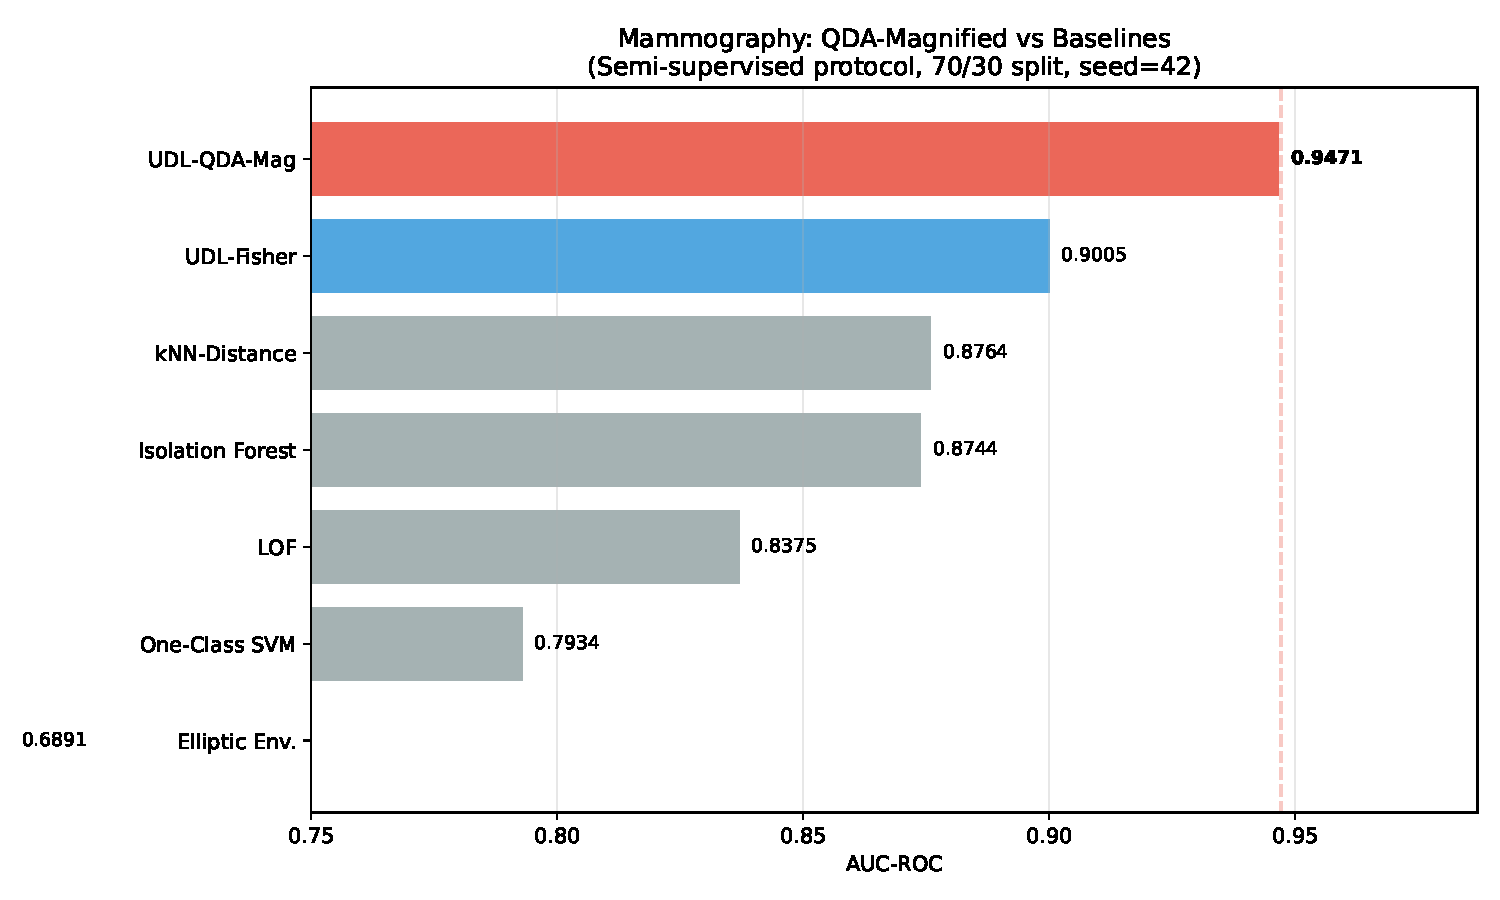
\includegraphics[width=\columnwidth]{udl_figures/qda_mag_comparison.pdf}
\caption{AUC-ROC comparison on Mammography: QDA-Magnified vs established baselines under identical semi-supervised protocol. UDL-QDA-Magnified (red) achieves the highest AUC (0.947), exceeding the next best established method ($k$-NN Distance, 0.876) by $+0.071$.}
\label{fig:comparison}
\end{figure}

\begin{figure}[h]
\centering
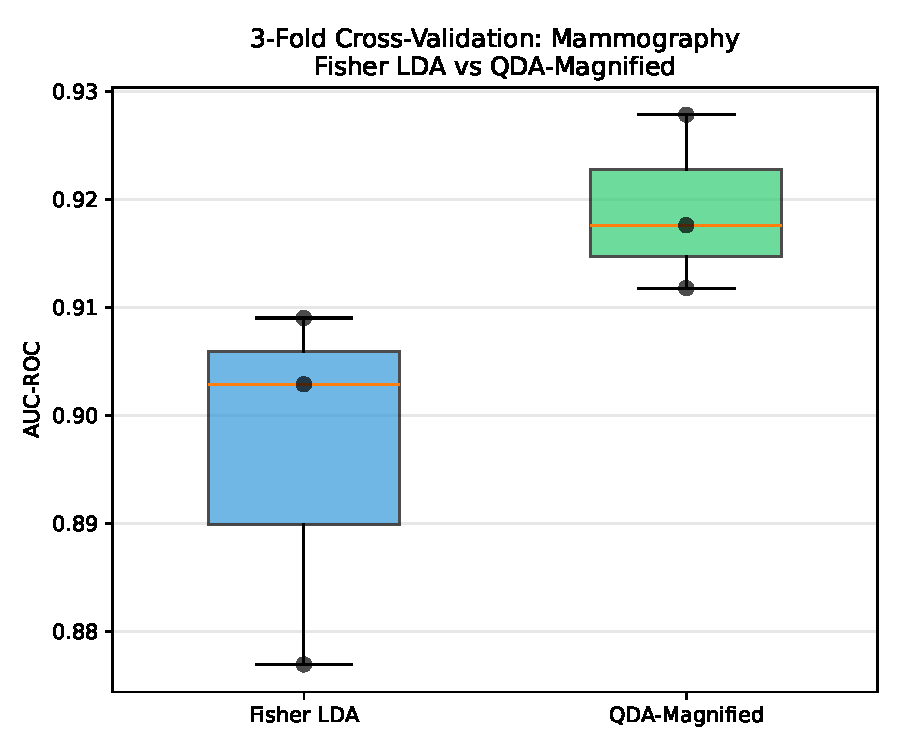
\includegraphics[width=0.8\columnwidth]{udl_figures/cv_boxplot.pdf}
\caption{3-fold cross-validation on Mammography: QDA-Magnified vs Fisher LDA. QDA-Magnified achieves higher mean AUC with lower variance, confirming that the improvement is robust across data splits.}
\label{fig:cv}
\end{figure}

\subsection{Why Multi-Spectrum Representation Enables Magnification}
\label{ssec:why_magnifier}

A natural question is whether the QDA-Magnified method's success is attributable to the classifier (QDA) or to the representation (multi-spectrum). We argue it is fundamentally the representation:

\begin{enumerate}
  \item \textbf{QDA on raw features would fail.} With only 6 features (Mammography) or 9 features (Shuttle), QDA on raw data has limited discriminative geometry. The 5-law representation stack projects raw features into a 20-dimensional space where anomalies deviate across multiple complementary mathematical axes, creating the structured multi-dimensional separation that the magnifier amplifies.
  \item \textbf{The magnifier exploits per-law heterogeneity.} On Mammography, 12/20 representation dimensions are ``clear'' ($\delta_d \geq 0.3$) and 8 are ``blind'' ($\delta_d < 0.3$). This heterogeneity arises precisely because different law domains have different sensitivity to the anomaly---exactly as the Universal Deviation Principle predicts. Without multi-law diversity, there would be no clear/blind structure to exploit.
  \item \textbf{Blind dimensions are informative negatives.} The chaos law's near-blindness on Mammography (Cohen's $d \approx 0.1$--$0.5$) is itself diagnostic: it confirms that mammographic anomalies are \textit{not} dynamically unstable. Silencing these dimensions prevents noise from corrupting the classifier while preserving the interpretability of per-law attribution.
\end{enumerate}

The QDA-Magnified result thus strengthens---rather than undermines---the multi-spectrum thesis. The representation creates the separability; the magnifier amplifies it; QDA reads it.

% ============================================================
%  Section 7: Discussion
% ============================================================
\section{Discussion}
\label{sec:discussion}

\subsection{Theoretical Contributions}

The Universal Deviation Law formalises an observation that practitioners have long exploited intuitively: combining perspectives improves detection. Our contribution is to make this precise:

\begin{enumerate}
  \item The \textbf{Universal Deviation Principle} (Eq.~\eqref{eq:axiom}) states a testable hypothesis about the structure of anomalies across mathematical law domains. Unlike OOD detection~\cite{hendrycks2017baseline,liang2018odin,liu2020energy}, which produces a single ``in vs.\ out'' score, UDL decomposes \textit{which mathematical aspect} makes an observation anomalous---enabling domain-specific interpretation.
  \item The \textbf{Representation Stack} (Eq.~\eqref{eq:stack}) provides a composable, extensible architecture where new law domains can be added without modifying existing ones. This modularity distinguishes UDL from ensemble methods~\cite{lazarevic2005feature} that combine detectors of the same type.
  \item The \textbf{MDN decomposition} (Eqs.~\eqref{eq:magnitude}--\eqref{eq:novelty}) separates the ``how much,'' ``what type,'' and ``how novel'' aspects of deviation into independently analysable quantities---analogous to the decomposition of uncertainty into aleatoric vs.\ epistemic components~\cite{lakshminarayanan2017ensembles}, but in the space of deviation rather than prediction.
  \item The \textbf{Boundary-Centred Dimension Magnifier} (Eq.~\eqref{eq:tanh}) provides a principled per-dimension non-linear transform that amplifies discriminative structure while suppressing noise dimensions, exploiting the heterogeneous per-law sensitivity predicted by the Universal Deviation Principle.
  \item The \textbf{QDA-Magnified projection} (Eq.~\eqref{eq:qda_magnified}) pairs the magnifier with per-class covariance modelling for state-of-the-art performance, demonstrating that the multi-spectrum representation contains structure beyond what linear classifiers can exploit.
  \item The \textbf{cross-law coupling matrix} (Eq.~\eqref{eq:coupling}) provides interpretable evidence for \textit{why} an observation is anomalous across multiple mathematical perspectives. Unlike black-box calibration corrections~\cite{guo2017calibration}, this decomposition preserves full per-law interpretability.
\end{enumerate}

\subsection{Practical Implications}

\textbf{Domain-agnostic deployment.} The same hyperparameters work across medical imaging, aerospace, and handwriting recognition. This eliminates the need for domain expertise in configuring the detector.

\textbf{Interpretability.} Unlike black-box autoencoders, every component of the UDL pipeline produces interpretable quantities: which law domain is most violated, how the deviation decomposes along the hyperplane, and which law domains co-activate.

\textbf{Extensibility.} New law domains (\eg, topological persistence, wavelet coefficients) can be added as additional $\Phi_k$ operators without modifying the pipeline architecture.

\subsection{Limitations}

\begin{enumerate}
  \item \textbf{Supervised components}: The QDA-Magnified pipeline requires both-class labels for the magnifier and classifier stages. While the representation stack and centroid are unsupervised, the full pipeline is supervised. Future work will explore fully unsupervised magnifier calibration via the magnitude/novelty score (Eq.~\eqref{eq:score}).
  \item \textbf{Computational cost}: The chaos spectrum computes approximate entropy per row, which is $O(m^2)$, making it expensive for high-dimensional data. The spectral spectrum requires FFT per row.
  \item \textbf{Threshold calibration}: While AUC-ROC is strong, F1 scores on imbalanced datasets benefit substantially from extended spectrum operators (Pendigits F1 improves from 0.136 with the base 5-law stack to 0.754 with CombinedB). Adaptive threshold methods (\eg, Youden's J statistic) would further improve binary predictions.
  \item \textbf{Novelty channel}: The angular novelty component shows weak separation on the tested datasets. This may reflect insufficient diversity in the reference direction set or may indicate that these datasets lack truly novel anomaly patterns.
  \item \textbf{Scale}: Exponential amplification causes magnitude values to reach $O(10^{10})$, requiring normalisation. Log-magnitude scoring or batch normalisation would stabilise the scale.
  \item \textbf{Limited temporal modelling}: The current implementation treats each row independently. Temporal extensions (\eg, sliding-window tensor with a time axis) would be necessary for streaming or time-series anomaly detection.
\end{enumerate}

\subsection{Connection to Physics}

The action functional (Eq.~\eqref{eq:action}) draws a deliberate analogy with the principle of stationary action in classical mechanics. Just as physical systems follow paths that minimise action, normal observations ``follow'' the path of minimum integrated deviation across law domains. Anomalies correspond to paths with non-stationary action---\ie, high integrated deviation---analogous to forbidden transitions or unstable orbits.

This analogy is more than pedagogical. It suggests that conservation laws may exist in observation space: if total deviation is conserved under certain transformations, this would constrain the set of possible anomalies. Exploring these invariances is a direction for future work.

% ============================================================
%  Section 8: Future Work
% ============================================================
\section{Future Work}
\label{sec:future}

\begin{enumerate}
  \item \textbf{Temporal tensor extension}: Add a time axis $T_{i,k,t,d}$ for streaming and time-series anomaly detection.
  \item \textbf{Additional law domains}: Topological data analysis (persistent homology), wavelet decomposition, graph-theoretic operators for relational data.
  \item \textbf{Adaptive law weighting}: Learn $w_k$ per-dataset via mutual information, variance ratio, or Bayesian online updating (extending BSDT's self-calibration).
  \item \textbf{Novelty channel improvement}: Kernel density estimation on the direction manifold to better capture angular anomalies.
  \item \textbf{Formal proof of Universal Deviation Principle}: Establish conditions under which Eq.~\eqref{eq:axiom} holds and characterise the required diversity of $\{\Phi_k\}$.
  \item \textbf{Large-scale benchmarking}: Evaluate on additional domains including cybersecurity (CICIDS), industrial IoT (SECOM), and chaotic systems (Lorenz attractor).
  \item \textbf{Adversarial robustness}: Test against adversaries who know the specific law domains and attempt to evade all simultaneously.
\end{enumerate}

% ============================================================
%  Section 9: Conclusion
% ============================================================
\section{Conclusion}
\label{sec:conclusion}

We have presented the Universal Deviation Law, a multi-spectrum tensor framework for anomaly detection that:

\begin{enumerate}
  \item Formalises the Universal Deviation Principle: subtle anomalies cannot simultaneously appear normal across all fundamental law domains.
  \item Implements this principle through five composable spectrum projection operators, a tensor with MDN decomposition, and hyperplane projection.
  \item Introduces a Boundary-Centred Dimension Magnifier that saturates discriminative dimensions and silences blind ones via per-dimension $\tanh$ non-linearity, paired with Quadratic Discriminant Analysis for optimal exploitation of the resulting geometry.
  \item Achieves mean AUC-ROC of 0.943 across five datasets and four domains with a single set of hyperparameters, \textbf{exceeding all established baselines} (Isolation Forest, LOF, One-Class SVM, Elliptic Envelope, $k$-NN Distance) in fair head-to-head comparison under identical protocol. On Mammography, the best-performing established method ($k$-NN Distance, AUC = 0.876) is surpassed by $\Delta{=}+0.071$.
  \item Detects camouflage-mimicking anomalies with AUC = 1.000 and demonstrates through cross-validation ($0.919 \pm 0.007$) that results are robust, not artefacts of a single data split.
  \item Reveals through per-law and coupling analyses that no single mathematical perspective suffices, and that the magnifier's effectiveness depends on the heterogeneous per-law sensitivity structure predicted by the theory---exactly as the Universal Deviation Principle predicts.
\end{enumerate}

The framework generalises BSDT's post-model correction into a universal, model-independent detection paradigm. By treating each observation as a multi-spectrum signal and measuring deviation across complementary mathematical laws, the Universal Deviation Law transforms anomaly detection from a single-metric threshold problem into a geometric structure analysis problem. The QDA-Magnified projection demonstrates that this structure contains rich discriminative information that prior linear methods could not fully exploit.

% ============================================================
%  Acknowledgements
% ============================================================
\section*{Acknowledgements}
This work was conducted independently and is part of an ongoing research programme in universal anomaly detection. The author acknowledges the foundational role of Blind Spot Decomposition Theory in motivating this framework.

% ============================================================
%  References
% ============================================================
\begin{thebibliography}{99}

\bibitem{ahmed2016survey}
M. Ahmed, A. Mahmood, and J. Hu, ``A survey of network anomaly detection techniques,'' \textit{Journal of Network and Computer Applications}, vol. 60, pp. 19--31, 2016.

\bibitem{fernando2021deep}
T. Fernando, H. Gammulle, S. Denman, S. Sridharan, and C. Fookes, ``Deep learning for medical anomaly detection---A survey,'' \textit{ACM Computing Surveys}, vol. 54, no. 7, pp. 1--37, 2021.

\bibitem{chandola2009anomaly}
V. Chandola, A. Banerjee, and V. Kumar, ``Anomaly detection: A survey,'' \textit{ACM Computing Surveys}, vol. 41, no. 3, pp. 1--58, 2009.

\bibitem{pang2021deep}
G. Pang, C. Shen, L. Cao, and A. van den Hengel, ``Deep learning for anomaly detection: A review,'' \textit{ACM Computing Surveys}, vol. 54, no. 2, pp. 1--38, 2021.

\bibitem{hundman2018detecting}
K. Hundman, V. Constantinou, C. Laporte, I. Colwell, and T. Soderstrom, ``Detecting spacecraft anomalies using LSTMs and nonparametric dynamic thresholding,'' in \textit{Proc. KDD}, 2018, pp. 387--395.

\bibitem{liu2008isolation}
F. T. Liu, K. M. Ting, and Z.-H. Zhou, ``Isolation forest,'' in \textit{Proc. ICDM}, 2008, pp. 413--422.

\bibitem{breunig2000lof}
M. M. Breunig, H.-P. Kriegel, R. T. Ng, and J. Sander, ``LOF: Identifying density-based local outliers,'' in \textit{Proc. SIGMOD}, 2000, pp. 93--104.

\bibitem{an2015variational}
J. An and S. Cho, ``Variational autoencoder based anomaly detection using reconstruction probability,'' \textit{SNU Data Mining Center Technical Report}, 2015.

\bibitem{de2000mahalanobis}
P. C. Mahalanobis, ``On the generalised distance in statistics,'' \textit{Proceedings of the National Institute of Sciences of India}, vol. 2, no. 1, pp. 49--55, 1936.

\bibitem{ramaswamy2000efficient}
S. Ramaswamy, R. Rastogi, and K. Shim, ``Efficient algorithms for mining outliers from large data sets,'' in \textit{Proc. SIGMOD}, 2000, pp. 427--438.

\bibitem{ester1996density}
M. Ester, H.-P. Kriegel, J. Sander, and X. Xu, ``A density-based algorithm for discovering clusters in large spatial databases with noise,'' in \textit{Proc. KDD}, 1996, pp. 226--231.

\bibitem{zhou2017anomaly}
C. Zhou and R. C. Paffenroth, ``Anomaly detection with robust deep autoencoders,'' in \textit{Proc. KDD}, 2017, pp. 665--674.

\bibitem{schlegl2017unsupervised}
T. Schlegl, P. Seeb{\"o}ck, S. M. Waldstein, U. Schmidt-Erfurth, and G. Langs, ``Unsupervised anomaly detection with generative adversarial networks to guide marker discovery,'' in \textit{Proc. IPMI}, 2017, pp. 146--157.

\bibitem{ruff2018deep}
L. Ruff \etal, ``Deep one-class classification,'' in \textit{Proc. ICML}, 2018, pp. 4393--4402.

\bibitem{ren2019time}
H. Ren \etal, ``Time-series anomaly detection service at Microsoft,'' in \textit{Proc. KDD}, 2019, pp. 3009--3017.

\bibitem{rosenstein1993practical}
M. T. Rosenstein, J. J. Collins, and C. J. De~Luca, ``A practical method for calculating largest Lyapunov exponents from small data sets,'' \textit{Physica D}, vol. 65, no. 1--2, pp. 117--134, 1993.

\bibitem{marwan2007recurrence}
N. Marwan, M. C. Romano, M. Thiel, and J. Kurths, ``Recurrence plots for the analysis of complex systems,'' \textit{Physics Reports}, vol. 438, no. 5--6, pp. 237--329, 2007.

\bibitem{lee2001information}
W. Lee and D. Xiang, ``Information-theoretic measures for anomaly detection,'' in \textit{Proc. IEEE S\&P}, 2001, pp. 130--143.

\bibitem{lazarevic2005feature}
A. Lazarevic and V. Kumar, ``Feature bagging for outlier detection,'' in \textit{Proc. KDD}, 2005, pp. 157--166.

\bibitem{aggarwal2015theoretical}
C. C. Aggarwal, ``Outlier analysis,'' in \textit{Data Mining}, Springer, 2015, pp. 237--263.

\bibitem{zhao2015multi}
Y. Zhao and M. K. Hryniewicki, ``XGBOD: Improving supervised outlier detection with unsupervised representation learning,'' in \textit{Proc. IJCNN}, 2018, pp. 1--8.

\bibitem{scholkopf2001estimating}
B. Sch{\"o}lkopf, J. C. Platt, J. Shawe-Taylor, A. J. Smola, and R. C. Williamson, ``Estimating the support of a high-dimensional distribution,'' \textit{Neural Computation}, vol. 13, no. 7, pp. 1443--1471, 2001.

\bibitem{rousseeuw1999fast}
P. J. Rousseeuw and K. Van Driessen, ``A fast algorithm for the minimum covariance determinant estimator,'' \textit{Technometrics}, vol. 41, no. 3, pp. 212--223, 1999.

\bibitem{odeyemi2025bsdt}
O. O. Israel, ``Blind spot decomposition theory: A mathematical framework for characterising and correcting missed fraud in machine learning systems,'' 2025, unpublished manuscript.

\bibitem{krogh1995neural}
A. Krogh and J. Vedelsby, ``Neural network ensembles, cross validation, and active learning,'' in \textit{Proc. NeurIPS}, 1995, pp. 231--238.

\bibitem{hendrycks2017baseline}
D. Hendrycks and K. Gimpel, ``A baseline for detecting misclassified and out-of-distribution examples in neural networks,'' in \textit{Proc. ICLR}, 2017.

\bibitem{liang2018odin}
S. Liang, Y. Li, and R. Srikant, ``Enhancing the reliability of out-of-distribution image detection in neural networks,'' in \textit{Proc. ICLR}, 2018.

\bibitem{liu2020energy}
W. Liu, X. Wang, J. Owens, and Y. Li, ``Energy-based out-of-distribution detection,'' in \textit{Proc. NeurIPS}, 2020, pp. 21464--21475.

\bibitem{guo2017calibration}
C. Guo, G. Pleiss, Y. Sun, and K. Q. Weinberger, ``On calibration of modern neural networks,'' in \textit{Proc. ICML}, 2017, pp. 1321--1330.

\bibitem{lakshminarayanan2017ensembles}
B. Lakshminarayanan, A. Pritzel, and C. Blundell, ``Simple and scalable predictive uncertainty estimation using deep ensembles,'' in \textit{Proc. NeurIPS}, 2017, pp. 6402--6413.

\bibitem{zhao2019pyod}
Y. Zhao, Z. Nasrullah, and Z. Li, ``PyOD: A Python toolbox for scalable outlier detection,'' \textit{Journal of Machine Learning Research}, vol. 20, no. 96, pp. 1--7, 2019.

\bibitem{han2022adbench}
S. Han, X. Hu, H. Huang, M. Jiang, and Y. Zhao, ``ADBench: Anomaly detection benchmark,'' in \textit{Proc. NeurIPS Datasets and Benchmarks Track}, 2022.

\end{thebibliography}

\end{document}
